\begin{figure}
    \begin{fullwidth}
    \centering
    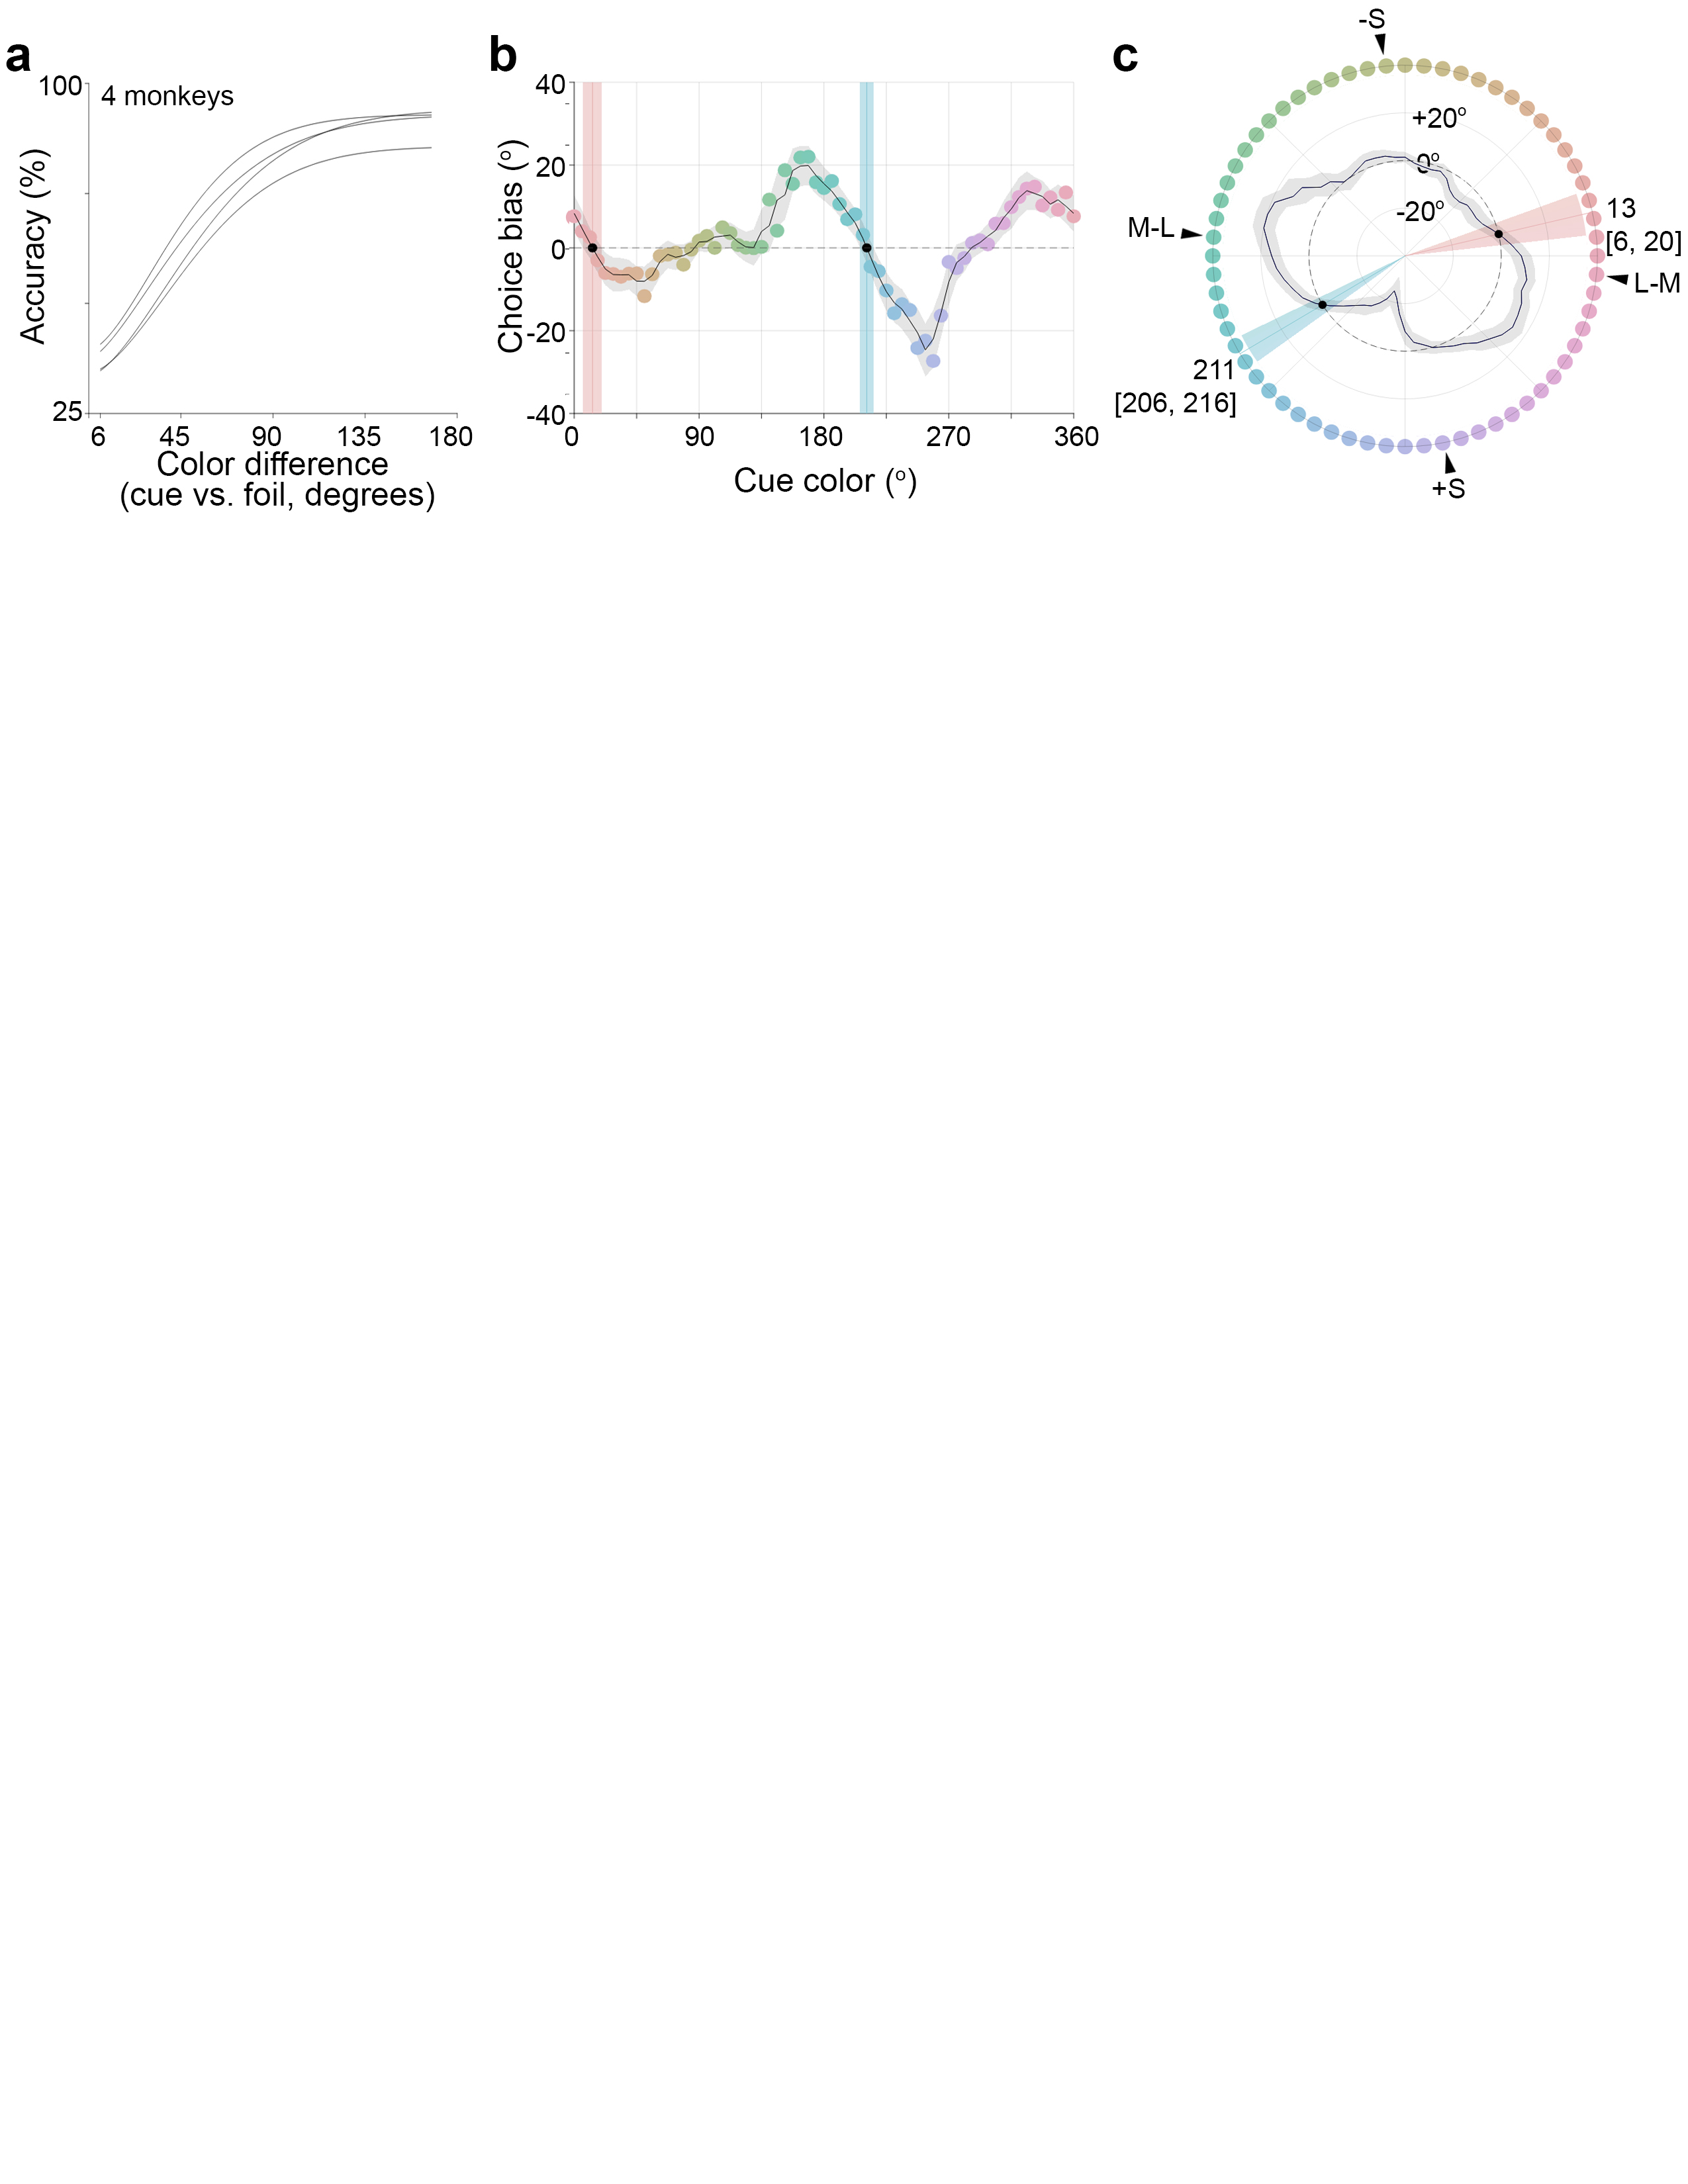
\includegraphics[width=\textwidth+4cm,trim={0 20cm 0 0},clip]{../Figures/flat/F2_CombinedMMResults_5.jpg}
    \caption{\textbf{Macaque monkeys appear to show two consensus color categories when the data are analyzed with a mixture model that computes the average distribution of the choices for each cue.}
	\textbf{a}, Psychometric functions for the four animals showing the accuracy of the matches as a function of the difference in hue angle between the cue and the foil that is closest in color to the cue. 
	The easiest trials were defined as those where the foil color nearest to the cue color were almost on the opposite side of the color circle. See SI Figure 2 for 95\% CI. 
	\textbf{b}, Mixture model results averaged across the four animals. The data were subsampled so that the same number of completed trials for each animal (24526) were included in the analysis. Error shading shows 95 \%CI. 
	The data recover two significant negative-slope zero-crossings (black dots), corresponding to two color categories. 
	\textbf{c}, Polar plot of the results in (b) with the zero crossings of the negative slope (following the trace counterclockwise) again indicated by black dots. The angle of the two inferred color categories [95 \% C.I.] are 13 [6, 20] (a peach color) and 211 [206, 216] (a teal color). }
    \label{fig:AvResults}
    \end{fullwidth}
\end{figure}

In the present experiments, the four animals performed well on the task, achieving a lapse rate of 7\%, 7.1\%, 5.8\%, 14.3\% (Figure 2a; the plots of individual animals showing 95\% CI are provided in SI Figure 2).
The results provided clear evidence of choice biases in all four animals (Figure 2).
But the inferred color categories, averaged across the four animals, do not support any of the predictions (Figure 2): the animals appeared to show two consensus color categories, not four as in humans. 
To the extent that the macaque is an accurate model of the human, these results show that the four color categories manifest in humans are not innate. 
The two category centers recovered in the monkeys, at angle 13 (a peach color) and 211 (a teal color), were not aligned with either of the cone-opponent mechanisms (arrowheads, Figure 2c); data for individual animals is shown in SI Figure 4).

\paragraph{Two possible explanations for choice biases in macaque monkeys}

\begin{figure}
    \begin{fullwidth}
    \centering
    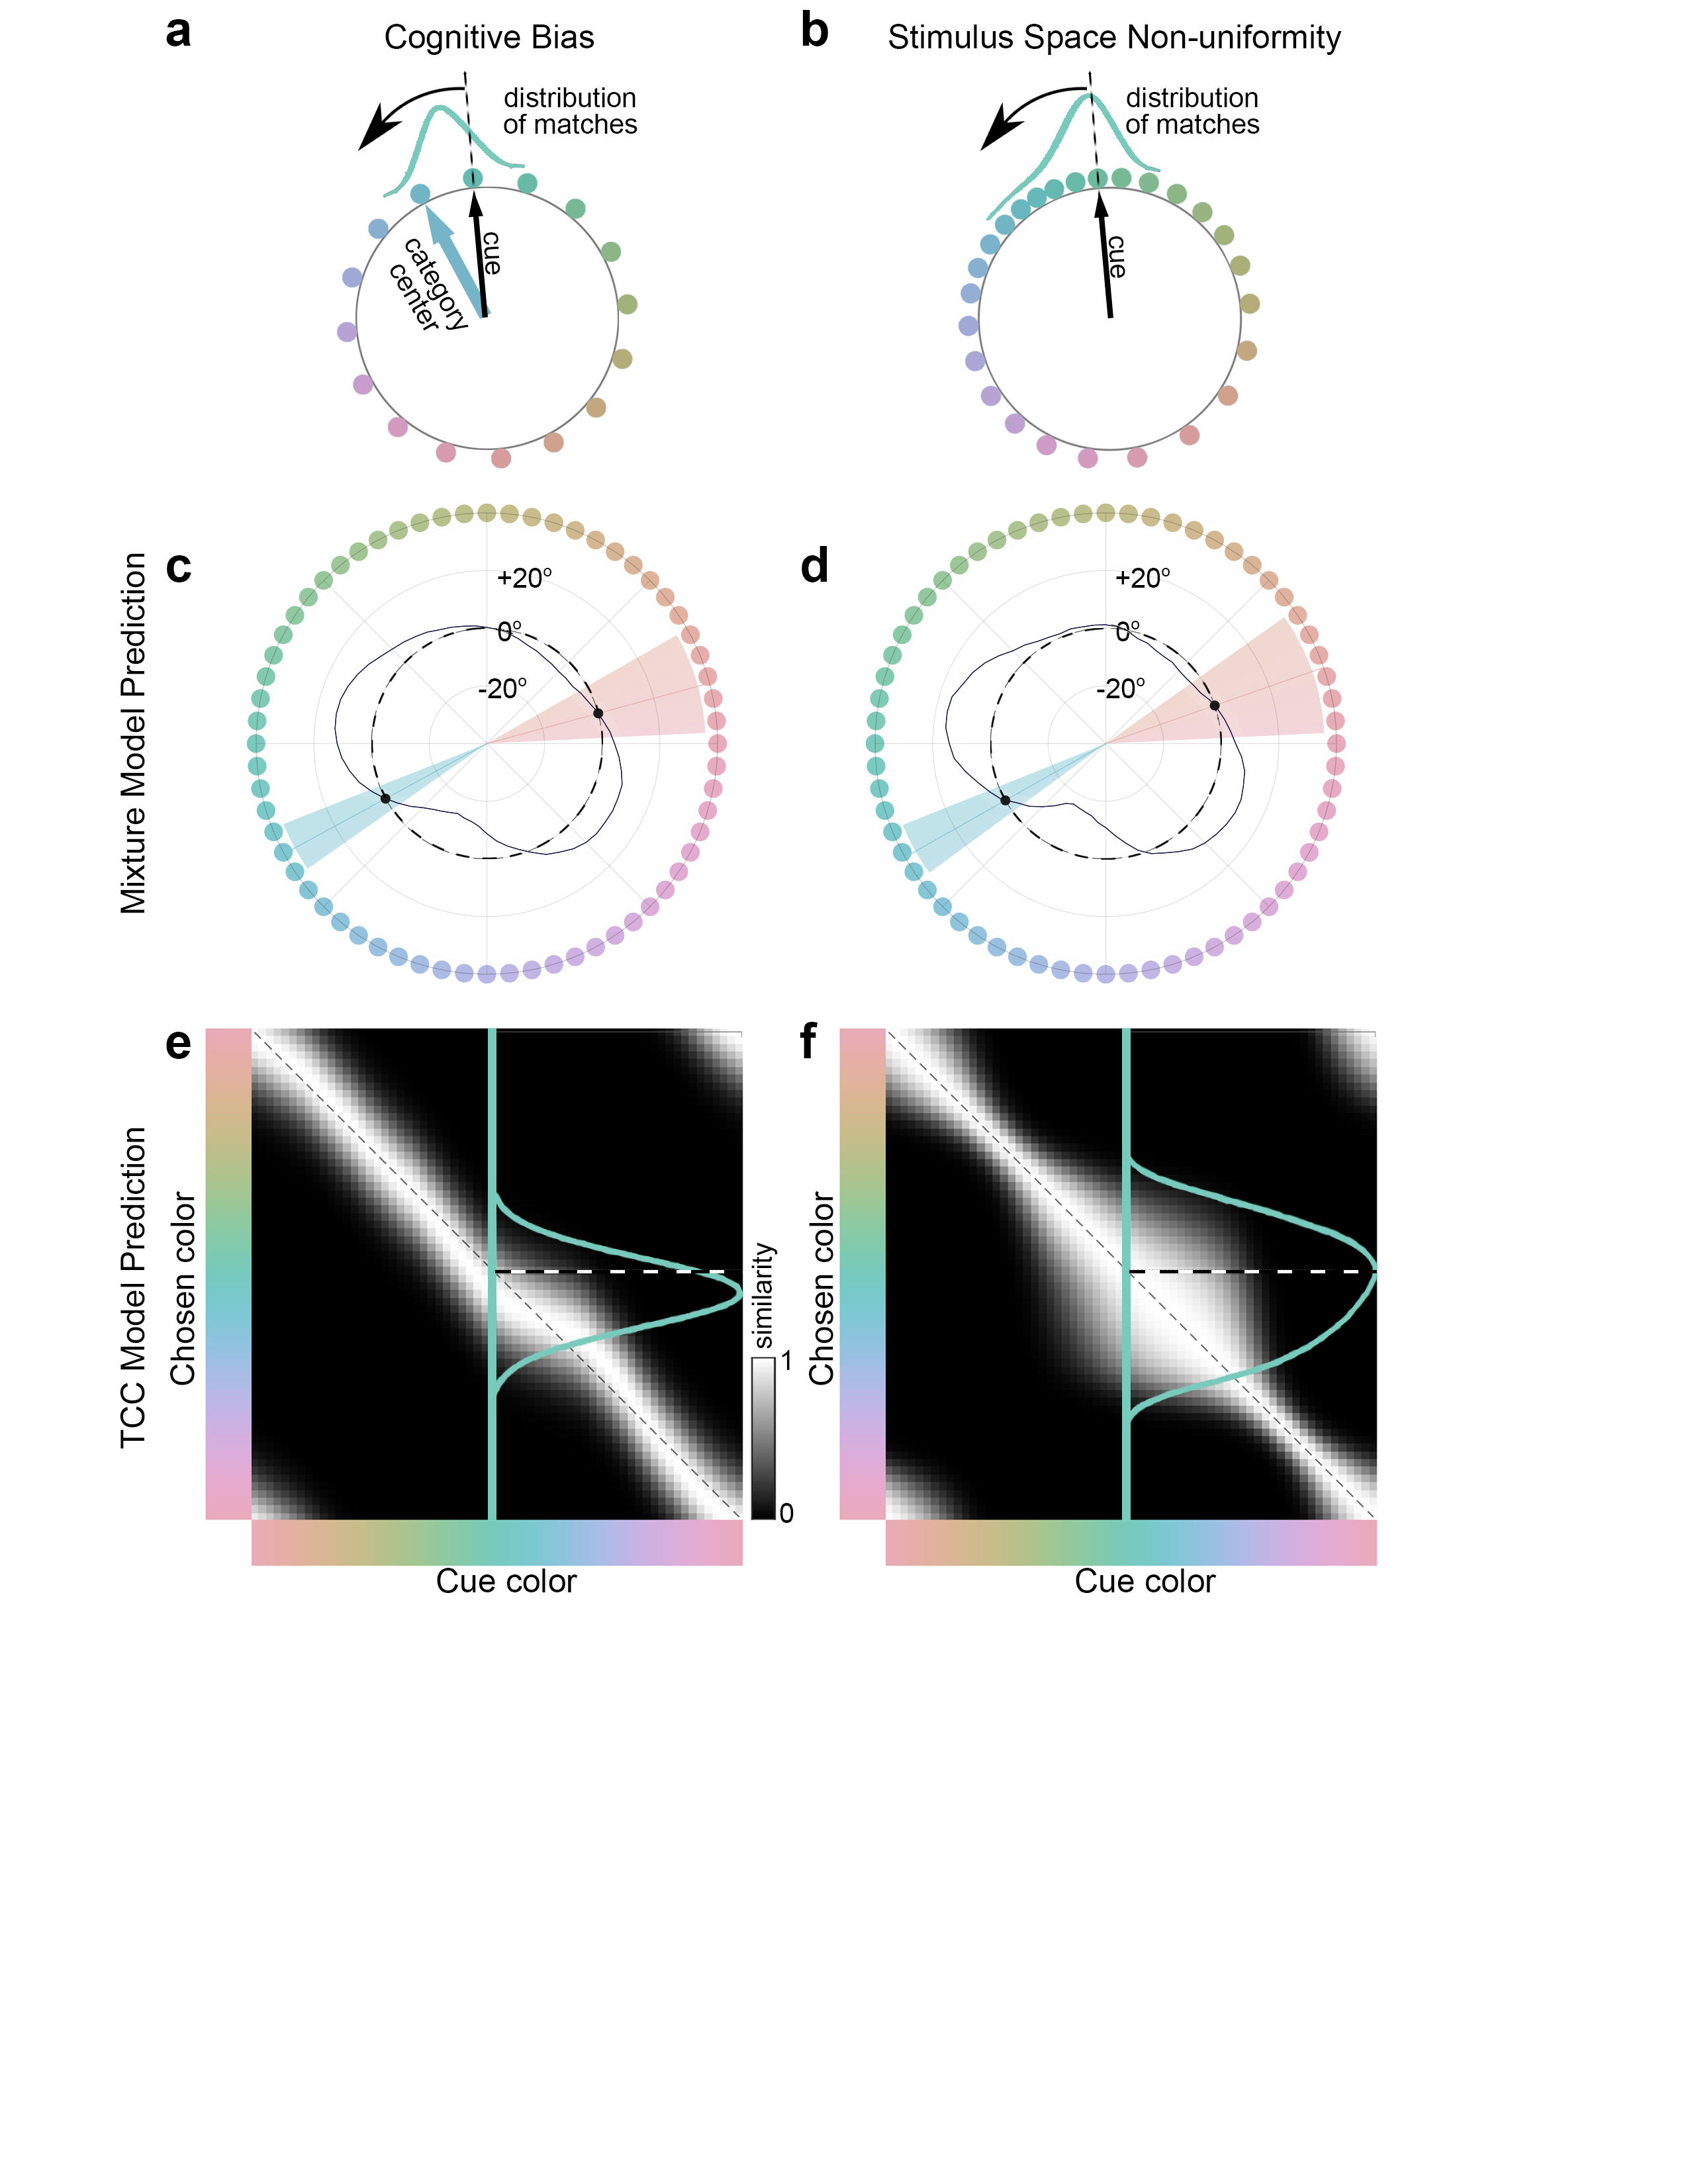
\includegraphics[width=\textwidth+4cm,trim={0 7cm 0 0},clip]{../Figures/flat/F3_TCCModel_6.jpg}
    \caption{\textbf{Behavioral data showing that putative color categories in macaque monkey can be explained by stimulus-space non-uniformities.} \textbf{a}, Color matches made by an agent with a cognitive color category, using a paradigm with stimuli that uniformly sample a truly uniform underlying perceptual color space (gray circle). 
	The distribution of matches comprises a similarity function (turquoise Gaussian) that is symmetric but with a peak deviated towards the category center. 
	\textbf{b}, Color matches made by an agent lacking cognitive color categories, using a paradigm with stimuli that non-uniformly sample a truly uniform underlying perceptual color space (gray circle). 
	The distribution of matches comprises a similarity function (turquoise asymmetric Gaussian) that is biased towards the more densely sampled region of the color space. 
	The bias arises simply because there are more choice options close to the cue color counterclockwise to the cue. 
	Note that in both a and b, the average of the distribution of matches is similarly deviated counterclockwise to the cue although the similarity functions differ. 
	\textbf{c}, Mixture-model analysis of a simulated data set with a cognitive bias. 
	\textbf{d}, Mixture-model analysis of a simulated data set with a stimulus space non-uniformity. 
	\textbf{e, f}, Similarity matrix for the same simulated data set analyzed in panel c, d. The axes depict the colors uniformly sampling CIELUV. The turquoise-colored traces shows the similarity functions for the cue in a,b.}
    \label{fig:TCCDemo}
    \end{fullwidth}
\end{figure}

The colors we used were defined by the International Commission on Illumination (CIE) to be approximately perceptually uniform. 
But it has long been recognized that there may be non-uniformities in the space \citep{stockman_colorimetry_2010}; some have argued that perceptual uniformity may be task-dependent or simply unattainable \citep{judd_ideal_1969}.

One might even suppose that if language influences color perception, as stipulated by the Sapir-Whorf hypothesis, then all color spaces generated by human observers could be shaped by language. 
Could the macaque consensus color categories be attributed not to a true cognitive category (Figure 3a) but to unrecognized distortions in the presumed uniform space of colors (Figure 3B)?
Both explanations could introduce biases in the distribution of matches.

The difference in the two explanations can be understood by considering the relationship between two neighboring colors. 
For the cognitive-bias account, there is an asymmetry between the colors if there is a category center nearby.
The color further from the category center will be more likely mistaken for the color closer to the category center than the other way around. 
Whereas for the non-uniform color space, there is no asymmetry in mismatches between neighboring colors. 
These two explanations would produce different shaped distributions of matches: the cognitive bias would yield the same width distribution for all cues around the color circle, but the peak of the distribution would deviate from the cue to varying degrees depending on the proximity of the cue to the category center. 
A stimulus space non-uniformity, meanwhile, would yield an asymmetric distribution that varies in width depending on sampling density of the underlying uniform color space, with regions that are relatively densely sampled having broader distributions. 
We refer to the distributions of matches for a cue, plotted in CIELUV, as its similarity function (hypothetical similarity functions shown in turquoise in Figure 3e and 3f).

To illustrate that the behavioral data could be explained by either a cognitive-bias account or a stimulus-space non-uniformity, we generated two sets of simulated data. 
One data set was generated with a simulation that used a uniform space and a bias arising from cognitive categories, and the other data set was generated with a simulation that used non-uniform sampling of an underlying uniform color space and no cognitive categories.
The data sets from both simulations gave rise to the same pattern of results when analyzed with a mixture model (Figure 3e and 3f).
These simulated data sets were chosen for illustration purposes because they correspond to the pattern of behavioral results (compare the simulated results with Figure 2c). 
The simulations show that the results recovered by the mixture model could be explained by stimulus space non-uniformities without appeal to cognitive color categories. 

To tease apart the possible underlying causes of the behavioral results, we extended the Target Confusability Competition (TCC) model \citep{schurgin_psychophysical_2020} (see Methods). 
The standard implementation of the TCC model assumes the same similarity function for each color. 
The extended version developed presently allows the similarity function to vary as a function of color. To distinguish the extended version of the model from the original, we call it TCC-v, "v" for "vary".
We introduce the concept of a similarity matrix, which captures the set of unique similarity functions for all colors in the space.
Let's consider three versions of the TCC-v model.
The simplest (“null”) model has the same two-parameter similarity function for each color, centered on the target color (this is conceptually equivalent to the original TCC model).  
The "cognitive bias" version of the model specifies similarity functions for each color with peaks that can deviate from the target color (Figure 3a). 
The result is a similarity matrix that has a band of constant width along the inverse diagonal but deviates to one side at color-category locations in the color space. 
The "stimulus-space non-uniformity" version of the model, meanwhile, has a similarity function for each target color that fixes the peak to the target color but where the angular distances between the colors can differ for different colors (Figure 3f). 
This results in a similarity matrix that is symmetric about the inverse diagonal, but which bulges out away from the diagonal at locations in the color space that are oversampled. 
The shape of the distribution of matches for a cue near the zero-crossing of the negative slope in the mixture model is indicated by the turquoise line in the cognitive bias and stimulus space non-uniformity versions of the TCC-v model. 
To recap, the similarity matrix in 3e is constructed using the same data as the polar plot in 3c; and the similarity matrix in 3f is constructed using the same data as the polar plot in 3d. 
These results show that different underlying mechanisms could explain the appearance of choice biases in color-matching tasks.

Next, we quantitatively compare the best fitting versions of each model to the behavioral data. 
To facilitate this comparison, we plot the behavioral data with a free-similarity version of the TCC-v model in which every cell in the similarity matrix is an independent model parameter (Figure 4a, 4b; the data for both panels are the same, centered on one or the other of the putative category centers recovered in the mixture model). 
The resulting matrix makes no assumptions about the underlying mechanisms that determine the similarity between any pair of stimuli. 
Now we can ask, are the data illustrated by the free similarity matrix better explained by the stimulus space non-uniformity model or the cognitive bias model? 
In other words, do the panels in Figure 4a and 4b show mirror symmetry with bulges about the diagonal (like Figure 3f) or asymmetry about the diagonal without bulges (like Figure 3e)? By visual inspection, the data are better explained by the stimulus space non-uniformity model, a conclusion affirmed by statistical tests. 

First, the stimulus space non-uniformity model provides a better fit of the data than the null model (Figure 4c). 
Second, the data are better explained by the stimulus-space non-uniformity model than the cognitive bias model (Figure 4d). 
These results strongly suggest that macaque monkeys do not have innate color categories. 
Again, if the macaque is an accurate model of the human, then the results imply that humans do not have innate color categories either. 

The data presented so far are for the four animals combined. 
The individual animals showed some idiosyncratic differences (SI Figure 4).
By mixture-model analysis, one animal showed not only the two consensus choice biases but also a third bias, for pea green (Figure 5a). 
The free similarity matrix for the data from this animal shows an asymmetry about the diagonal at this location in the color space (Figure 5b), showing that this animal has a cognitive bias for pea-green in addition to the consensus biases driven by stimulus-space non-uniformities (free similarity matricies for all animals shown in SI Figure 5). 
These results show that macaque monkeys have the potential to form cognitive color biases, and that the TCC-v model can recover them. The existence of cognitive biases in individual animals is consistent with prior work that observed different patterns of color-matching behavior in two animals using the continuous-matching task that likely reinforces idiosyncratic acquired biases \citep{panichello_error-correcting_2019}.


\begin{figure}
    \begin{fullwidth}
    \centering
    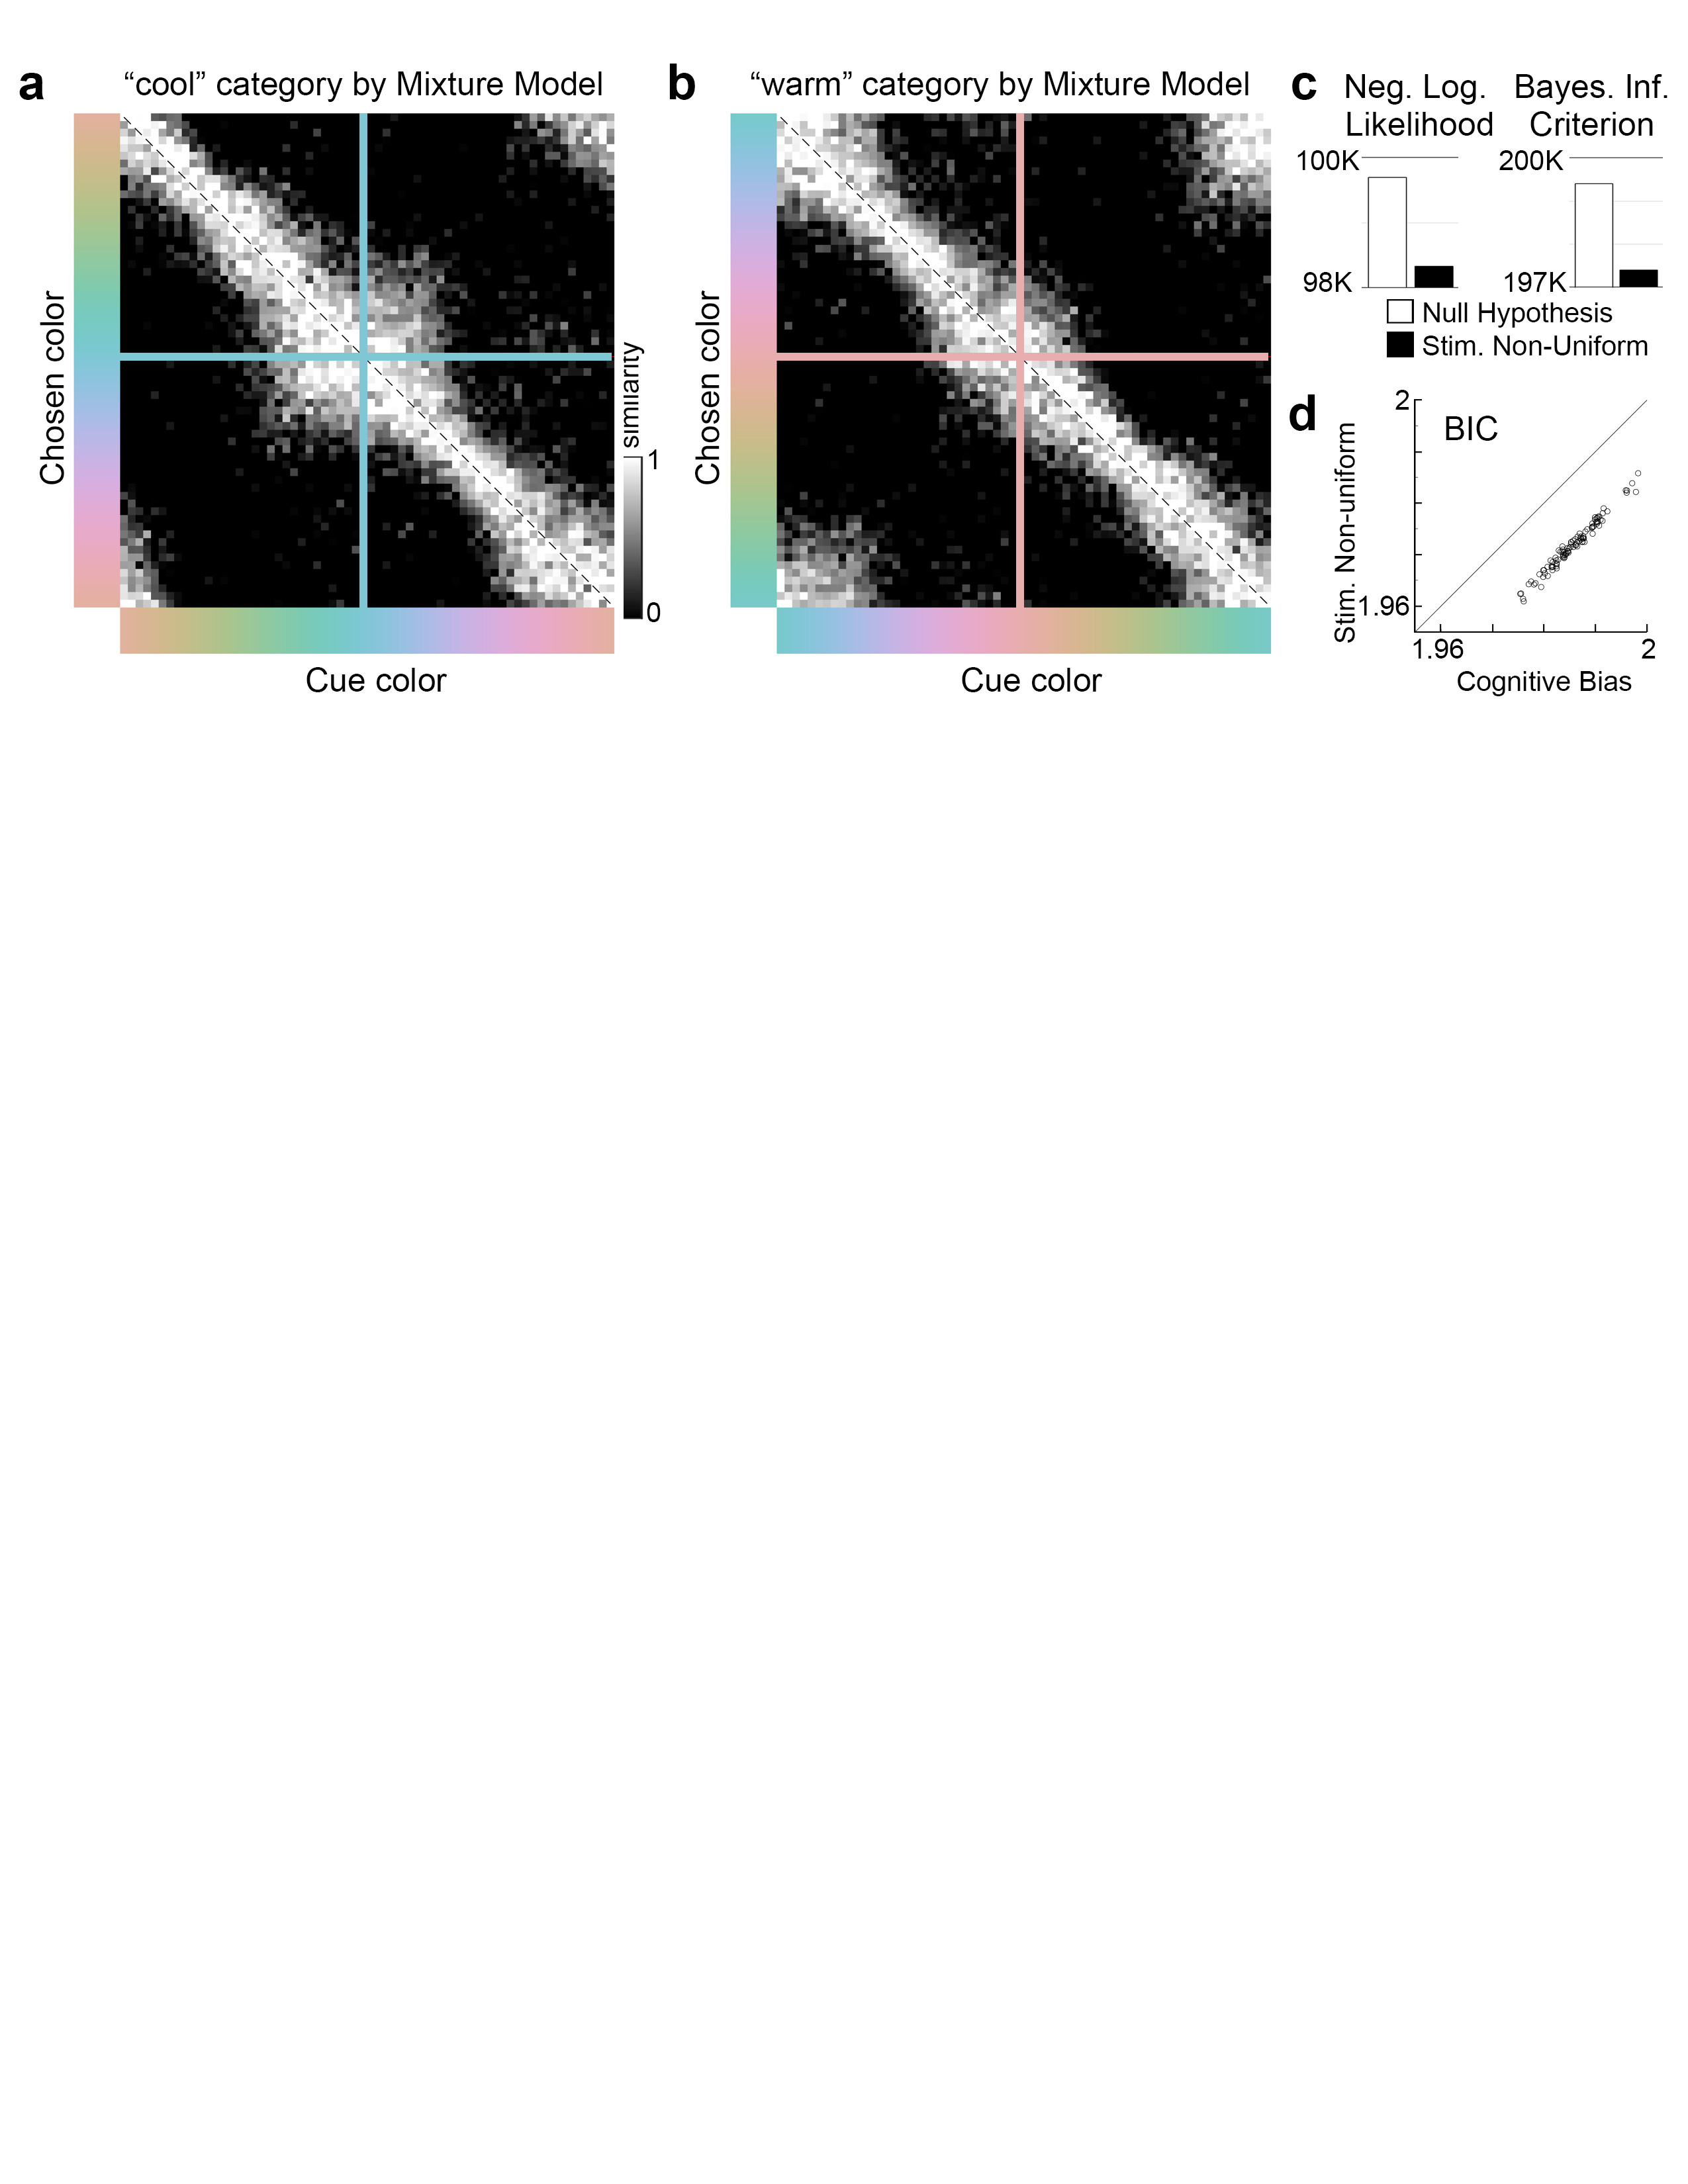
\includegraphics[width=\textwidth+4cm,trim={0 19cm 0 0},clip]{../Figures/flat/F4_TCCResults_3.jpg}
    \caption{\textbf{Similarity matrices for behavioral data averaged across four monkeys show that stimulus-space non-uniformities explain apparent color categories in monkeys.}
    \textbf{a}, Data are centered on the teal-colored category recovered in the mixture model. 
	\textbf{b}, Data are centered on the peach-colored category recovered in the mixture model. 
	\textbf{c}, Negative Log Likelihood (left) and Bayesian Inference Criterion (BIC, right) of the fit of the null model and the stimulus-space non-uniformity model. 
	\textbf{d}, BIC estimates of the fit provided by the stimulus-space non-uniformity model were always lower than BIC estimates of the fit for the cognitive bias model for 100 bootstrap repeats of the analysis (note that the stimulus space non-uniformity model and the cognitive bias model have the same number of parameters). 
	Each data point shows one bootstrap repeat of the analysis. For each boostrap repeat, the number of trials for each animal were the same, set by the animal that completed the smallest total number of completed trials, and that number of trials was drawn with replacement from the total number of completed trials for each animal. 
    } 
    \label{fig:TCCOutput}
    \end{fullwidth}
\end{figure}

\begin{figure}
    \begin{fullwidth}
    \centering
    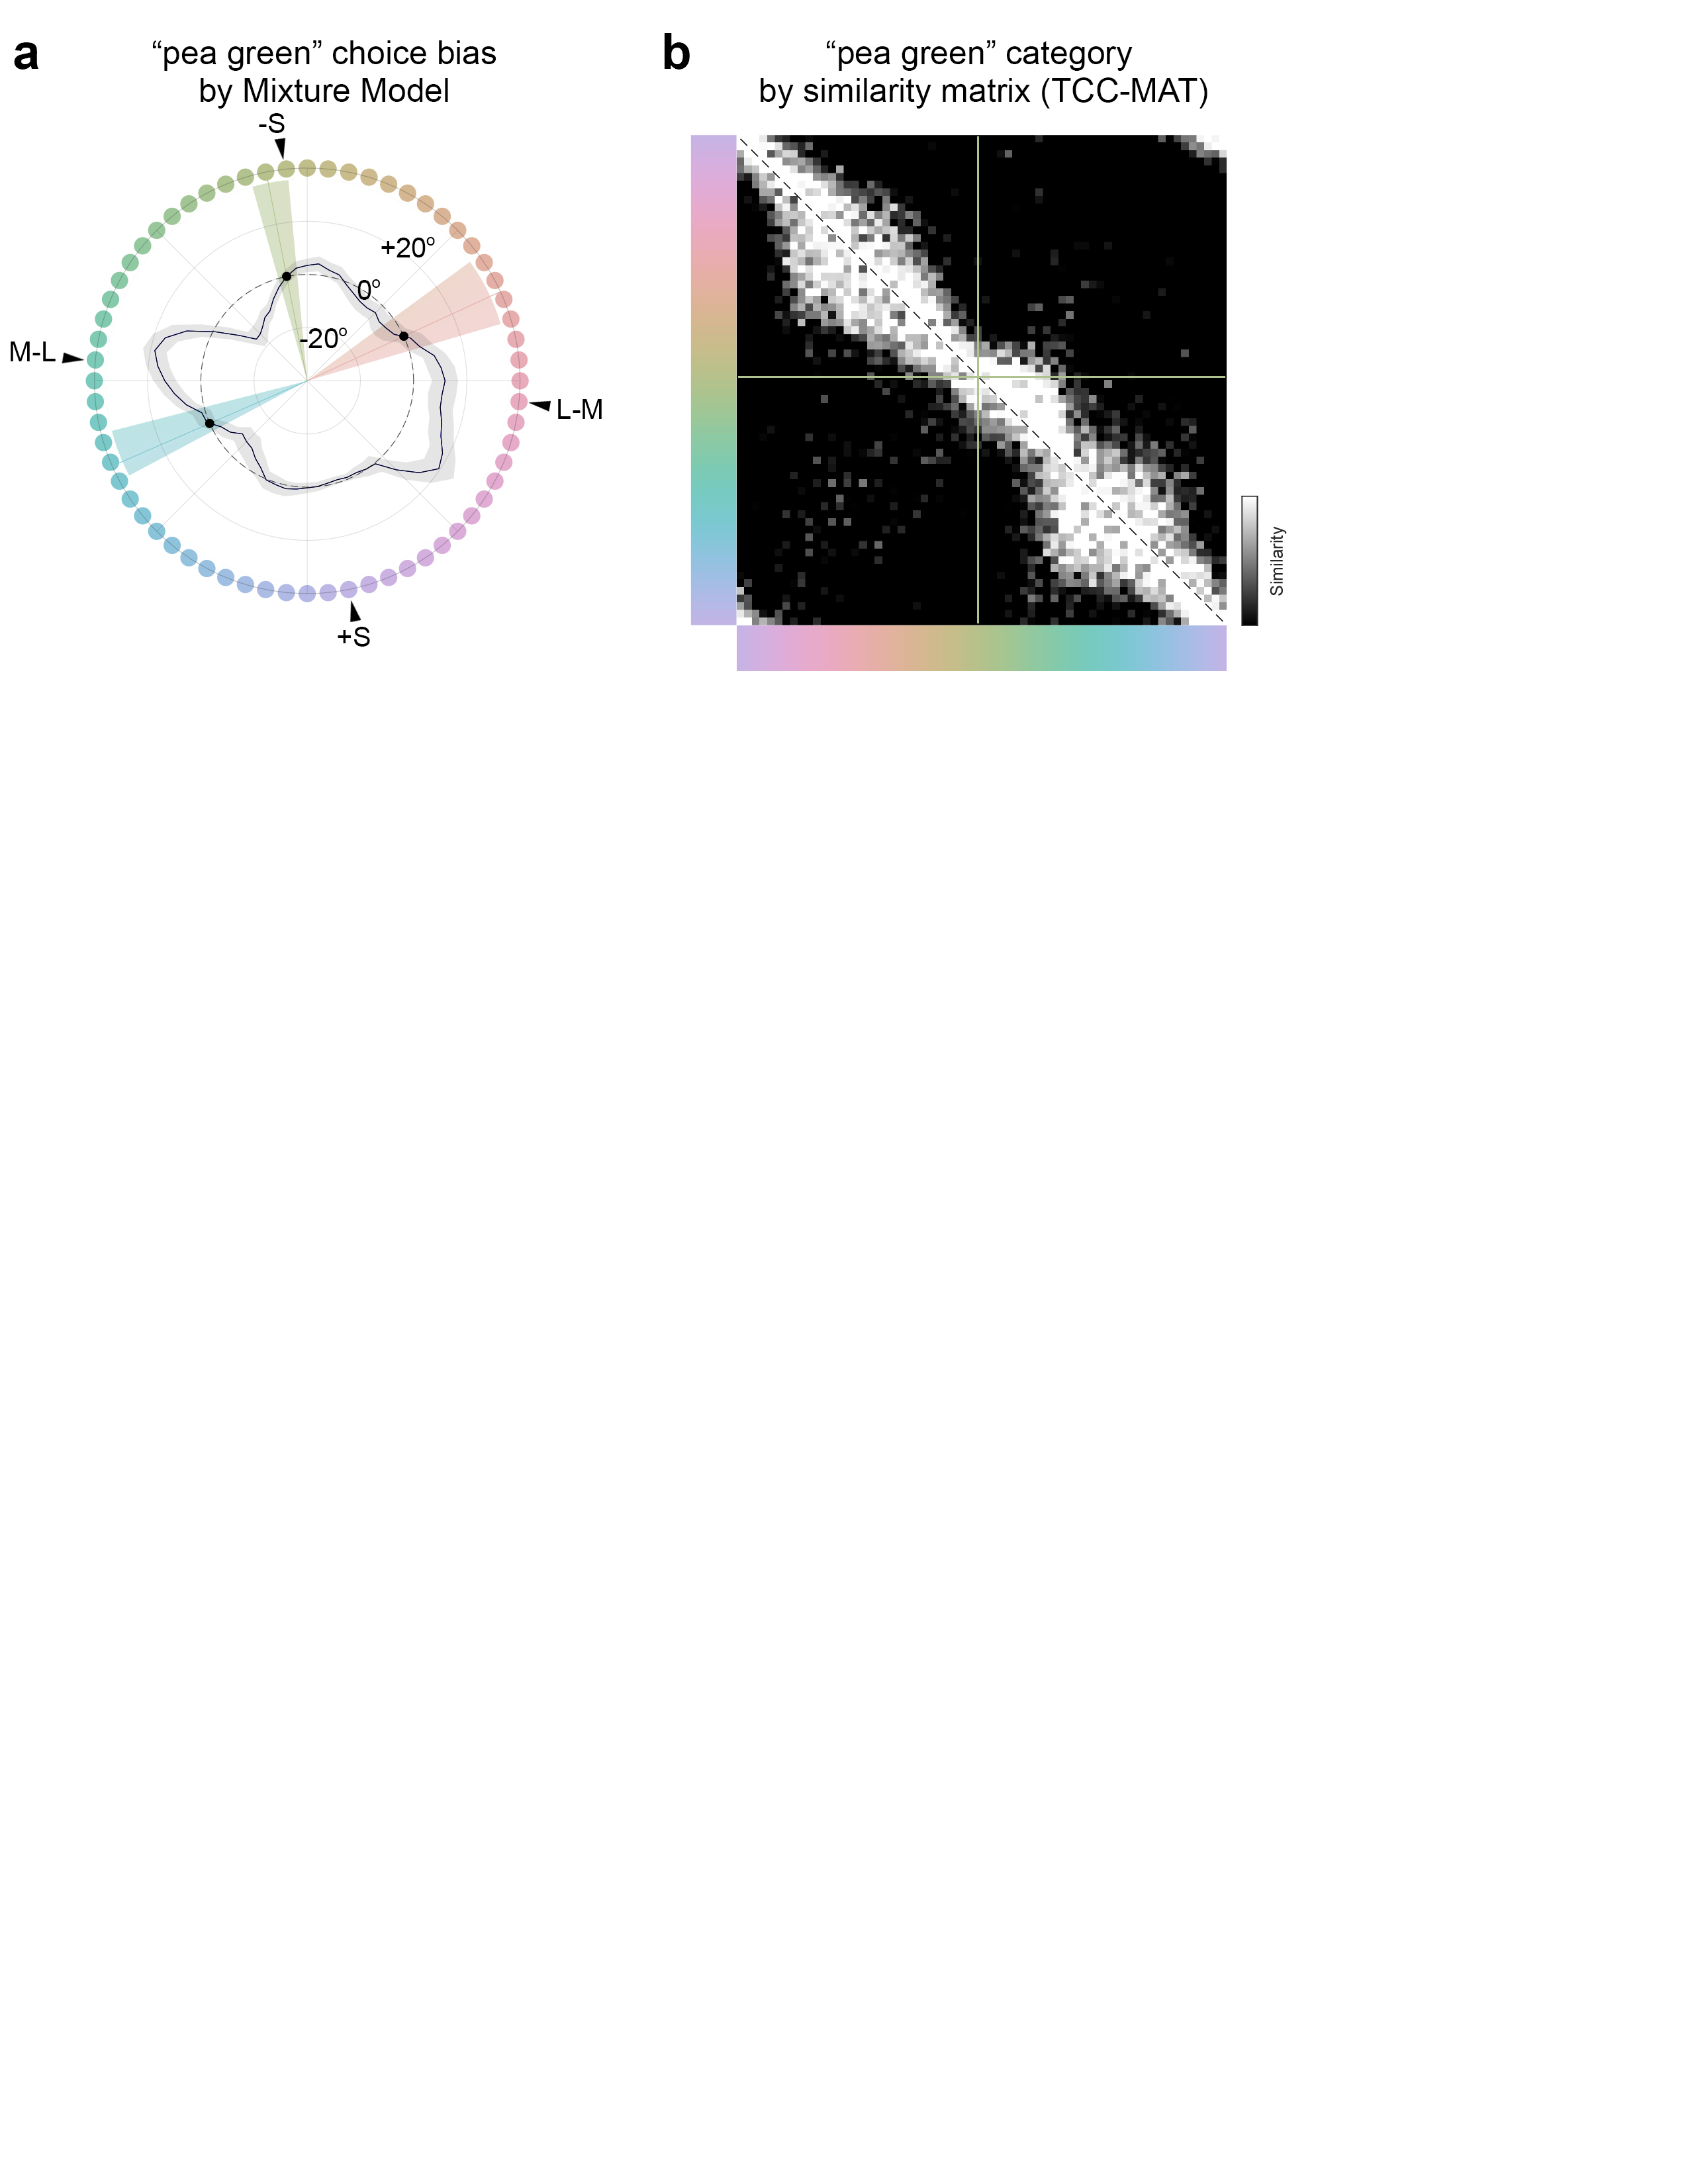
\includegraphics[width=\textwidth+4cm,trim={0 18cm 0 0},clip]{../Figures/flat/F5_CastorCogBias_6.jpg}
    \caption{\textbf {Color-matching data for one monkey showing evidence for a cognitive color category bias.} 
    \textbf{a}, Mixture-model analysis (same format as Figure 2c). 
	\textbf{b}, Free-similarity matrix (same format as Figure 4a,b) with an asymmetry in the green region indicated by the cross.}
    \label{fig:IndiDataCogBias}
    \end{fullwidth}
\end{figure}

\begin{figure}
    \begin{fullwidth}
    \centering
      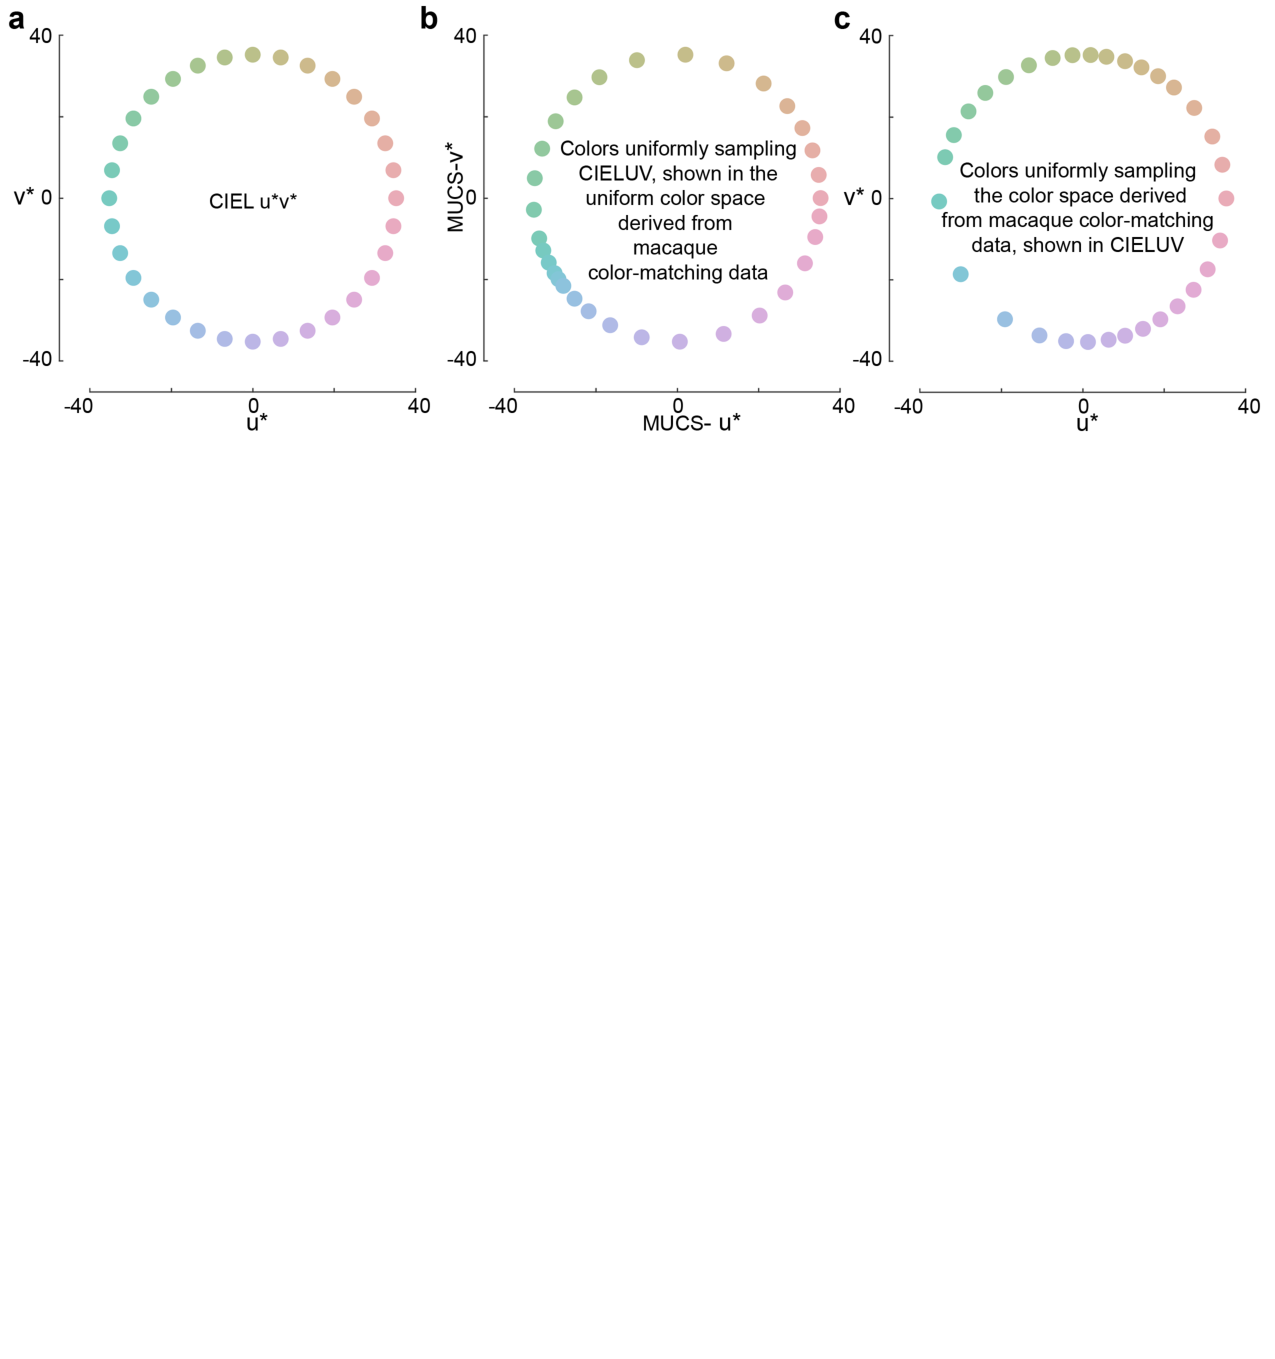
\includegraphics[width=\textwidth+4cm,trim={0 15cm 0 0},clip]{../Figures/flat/F6_ColSpace_2}
           \caption{\textbf{Perceptually uniform color space derived from the color-matching data in macaque monkeys.} 
			\textbf{a}, CIELUV color space with 64 color samples at even intervals in hue angle. 
			\textbf{b}, The same color samples plotted in the uniform color space derived from macaque monkeys; note that the axes are not CIELUV but MUCS (macaque uniform color space). 
			\textbf{c}, Colors sampled from evenly from the uniform color space derives from macaque monkeys, projected into CIELUV.}
		\label{fig:MACBEHcolorspace}
    \end{fullwidth}
\end{figure}


\paragraph{A perceptually uniform color space unconfounded by language}

The behavioral data in macaques provide a rare opportunity to reconstruct a perceptually uniform color space unconfounded by language.
We computed, empirically, a transformed color space such that the macaques would, on average, show no choice bias. 
We refer to this space as the Macaque Uniform Color Space (MUCS). 
When colors evenly sampled from the CIELUV space (Figure 6a) are plotted within this macaque-derived uniform color space, colors are bunched around the teal part of the space, and to a lesser extent, around the peach-colored part of the space (Figure 6b). 
We can also take colors sampled at uniform intervals in MUCS and project them into CIELUV (Figure 6c). This arrangement shows relative bunching around the yellows and purples, which correspond to the colors of the poles of the S-cone-opponent axes. 

The mixture-model results in macaque monkeys are strikingly different from those in humans, insofar as the data in humans consistently recover evidence of four consensus categories, while the data in macaque monkeys show evidence of only two consensus categories. But the data in the two species are similar in one regard: they both show repeller points aligned with the poles of the S-cone axis (compare the zero crossings of the positive slopes in Figure 1e with those in Figure 2c). \citep{skelton_biological_2017,bae_why_2015,panichello_error-correcting_2019}. These results raise the possibility that non-uniformities emerge in CIELUV because the contribution of S-cone signals to color perception has not been accurately estimated. Such an inaccuracy may reflect a discrepancy between measurements at threshold (as used in the generation of CIELUV) versus above threshold (as used in the present work), or the amplification of subcortical S-cone signals by the cortex \citep{RN655}.

The present results are consistent with the idea that color ordering and the capacity to form color categories is innate, but not the specific color categories themselves. Contrary to longstanding arguments in empirical philosophy \citep{RN18743}, perception by itself  appears to be insufficient to generate the consensus color categories evident in many studies of human color categorization.
If color categories are not innate, where do they come from? We wonder whether color categories reflect the behavioral relevance of colors in the world; the relevance of things is partially culturally determined, introducing a role for language in shaping consensus color categories. Given that color categories can be learned, as evident in at least one macaque in our study (Figure 5) and two macaques in another study \citep{panichello_error-correcting_2019}, the introduction of language provides a mechanism by which cultures can form consensus about color categories. For example, the parts of scenes labeled as objects by human observers are more likely to be warm colored while backgrounds are more likely to be cool colored \citep{rosenthal_color_2018}, and these statistics predict universal patterns in color naming \citep{gibson_color_2017}. We speculate that the choice biases in humans, which include at least double the number of consensus choice biases in monkeys, likely reflect cognitive biases, and that these cognitive biases achieve consensus through shared behavioral relevance and communication \citep{RN18511,RN18514,RN18602}. 
